%# -*- coding: utf-8-unix -*-
% !TEX program = xelatex
% !TEX root = ../thesis.tex
% !TEX encoding = UTF-8 Unicode

\chapter{系统实现}

在前两个章节中,已经进行了系统的需求分析并明确了系统设计的方法,
本章将按照前文所确定的需求和设计,利用软件开发工具和相关技术完成
基于iOS的任务计划及时间管理系统

\section{系统的实现环境}
本系统开发采用的IDE为 Xcode,数据库为Core Data,主要开发语言为 Swift。
由于本系统采用的Swift版本为Swift 5 故需要iOS 8.0以上的操作系统才可以使用, \parencite{wals2018mastering}
考虑到iOS新版本的普及率,是可以接受的。

\section{系统模块的实现}
本程序主要涉及事件管理、项目管理、任务管理、精力分析、行为管理五个模块,
每个模块都有众多功能,以下仅对这五个模块中的主要功能的实现进行介绍。

\subsection{事件管理模块}
根据系统设计阶段的需求,事件管理模块应能正确访问系统自带的日历
并能对其中的事件进行添加、删除和修改,并将相关的数据保存到系统的EventStore中,
以实现系统自身基于iCloud的同步。在初次进入主界面时,请求对系统日历的读写权限,
若已经授权则在后台读取今天的日程并进行展示,不影响主线程的操作,同时提供添加日程和编辑日程的功能。

由于用户可能随时关闭对该应用对日历的访问权限,故每次都需要对日历权限进行检查,若没有授权则进行请求,
如图\ref{fig:new_event_no_access}和\ref{fig:new_event}所示。

\begin{lstlisting}[language={Swift}, caption={请求日历权限代码逻辑}]
	func checkEventAuthorizationStatus() {
		let status = EKEventStore.authorizationStatus(for: .event)
		switch status {
		case .notDetermined:
			requestAccessToEvent()
		case .authorized:
			break
		default:
			break
		}
	}
	func requestAccessToEvent() {
		store.requestAccess(to: EKEntityType.event, completion: {
			(accessGranted: Bool, error: Error?) in
			if accessGranted == true {
				...
			}
		})
	}
\end{lstlisting}

\begin{figure}[!htbp]
	\centering
	\makebox[\textwidth]{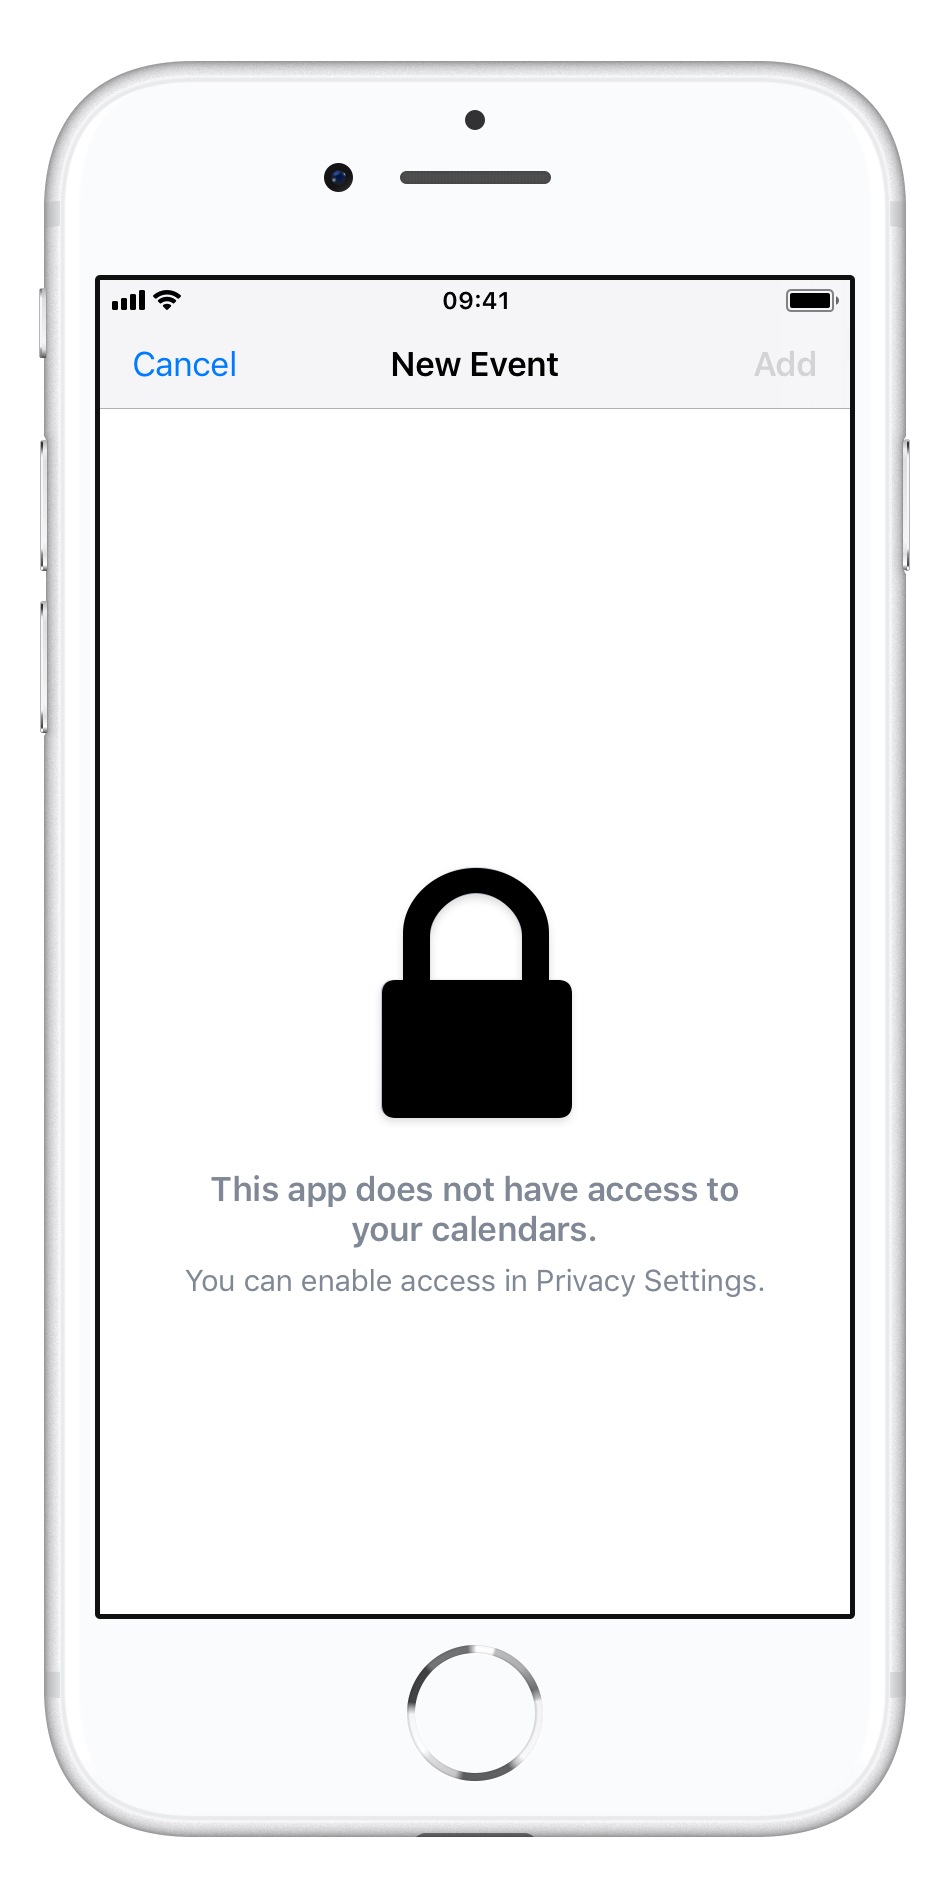
\includegraphics[height=10cm]{figure/system/new_event+no_access}}
	\caption{未获取日历权限创建新事件截图}
	\label{fig:new_event_no_access}
\end{figure}

\begin{figure}[!htbp]
	\centering
	\makebox[\textwidth]{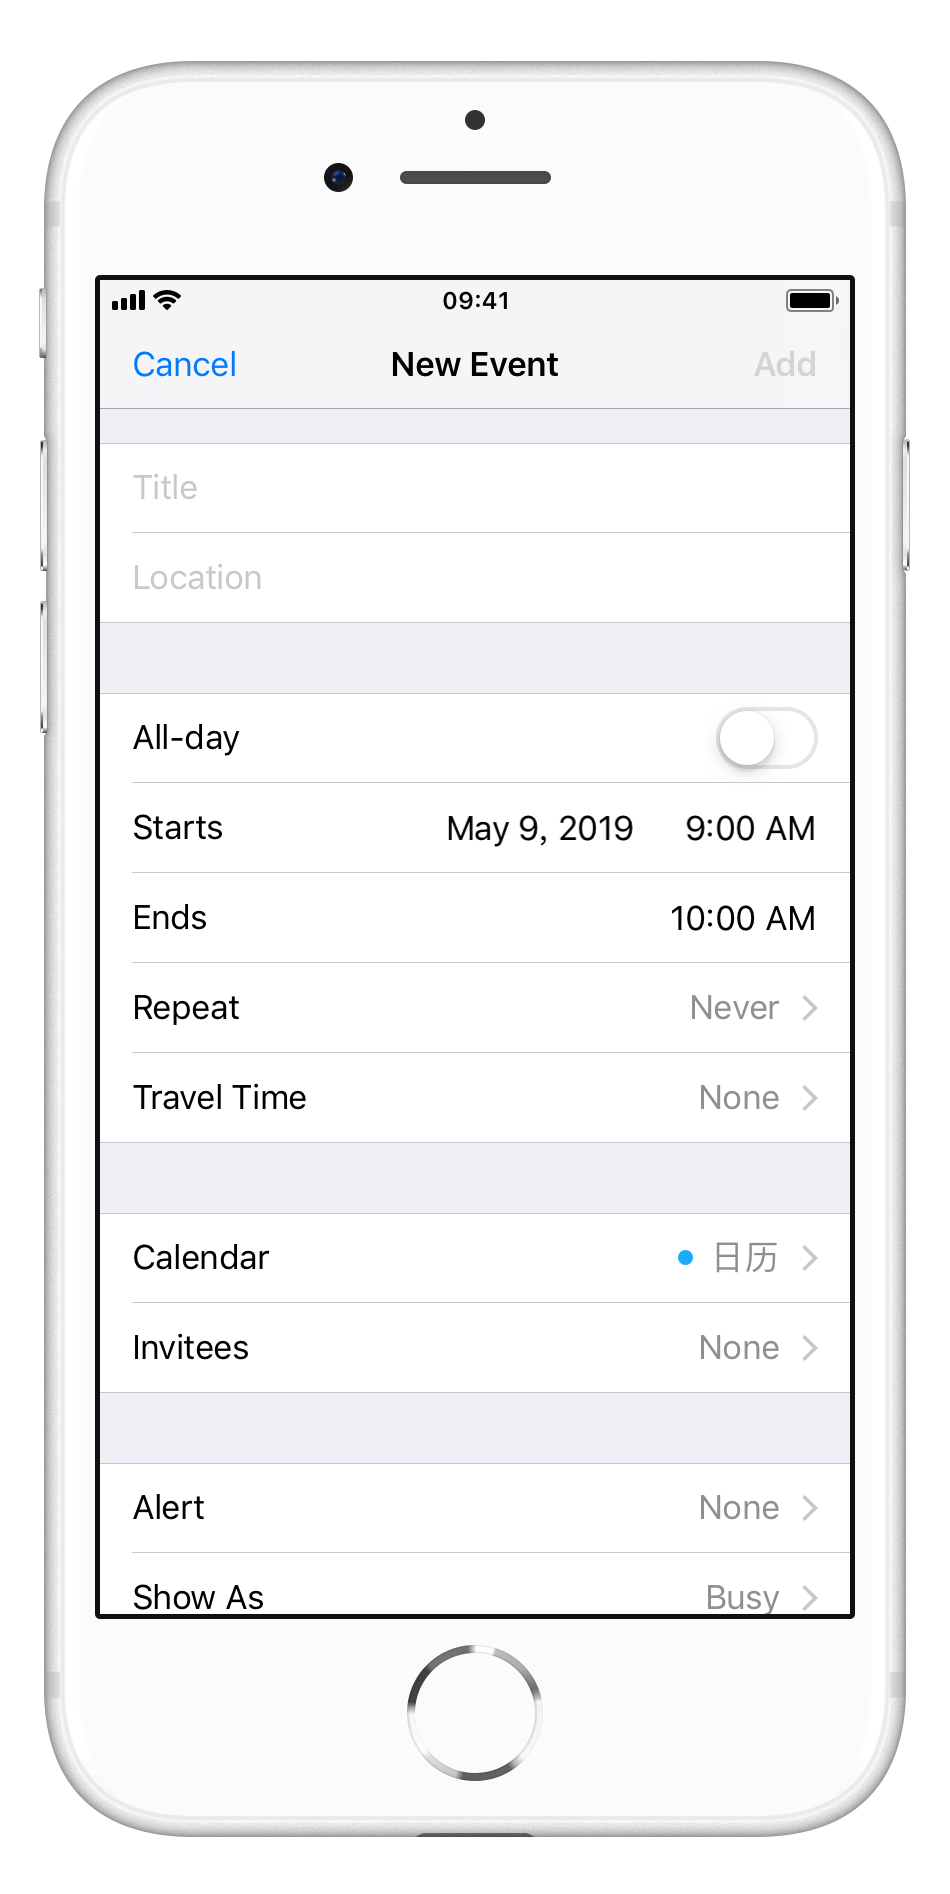
\includegraphics[height=10cm]{figure/system/new_event}}
	\caption{已获取日历权限创建新事件截图}
	\label{fig:new_event}
\end{figure}

\subsection{任务管理模块}
用户可以添加任务、修改任务、删除任务或将任务标记为已完成,
在Inbox(收件箱)\footnote{此处的收件箱并不是指邮件系统的收件箱,而是GTD理念中的将待办事项整合起来的地方。}
中,用户可以通过系统自带Siri功能\footnote{目前采用的是一种曲线救国的方法,即通过EventKit访问系统自带的提醒事项来达到类似Siri直接添加的效果。}
无需说应用名称,就可以添加新任务,这大大减少了输入带来的不便。
~\\
~\\
~\\
\begin{lstlisting}[language={Swift}, caption={请求提醒事项权限并导入系统代码逻辑}]
	func checkReminderAuthorizationStatus() {
        let status = EKEventStore.authorizationStatus(for: .reminder)
        switch status {
        case .notDetermined:
            requestAccessToReminder()
        case .authorized:
            loadReminders()
        default:
            break
        }
    }
    func requestAccessToReminder() {
        store.requestAccess(to: EKEntityType.reminder, completion: {
            (accessGranted: Bool, error: Error?) in
            if accessGranted == true {
                DispatchQueue.main.async(execute: {
                    self.loadReminders()
                    self.updateTasks()
                })
            }
        })
    }
    func loadReminders() {
        let predicate: NSPredicate? = store.predicateForReminders(in: [store.defaultCalendarForNewReminders()!])
        if let aPredicate = predicate {
            store.fetchReminders(matching: aPredicate, completion: {(_ reminders: [EKReminder]?) -> Void in
                for reminder: EKReminder? in reminders ?? [EKReminder?]() {
                    if(!reminder!.isCompleted) {
                        let task = Task(context: self.context)
                        task.title = reminder?.title
                        task.notes = reminder?.notes
                        task.dueDate = reminder?.dueDateComponents?.date
                        try? self.store.remove(reminder!, commit: true)
                        try? self.context.save()
                    }
                }
            })
        }
    }
    func updateTasks() {
        let request: NSFetchRequest<Task> = Task.fetchRequest()
        let predicate = NSPredicate(format: "project == %@", sourceProject ?? 0)
        request.predicate = predicate
        tasks = try! context.fetch(request)
    }
\end{lstlisting}

如图\ref{fig:inbox_no_split}所示,这项功能只会导入系统提醒事项中未完成的任务,避免数据过多导致缺失重点。

\begin{figure}[!hbp]
	\centering
	\makebox[\textwidth]{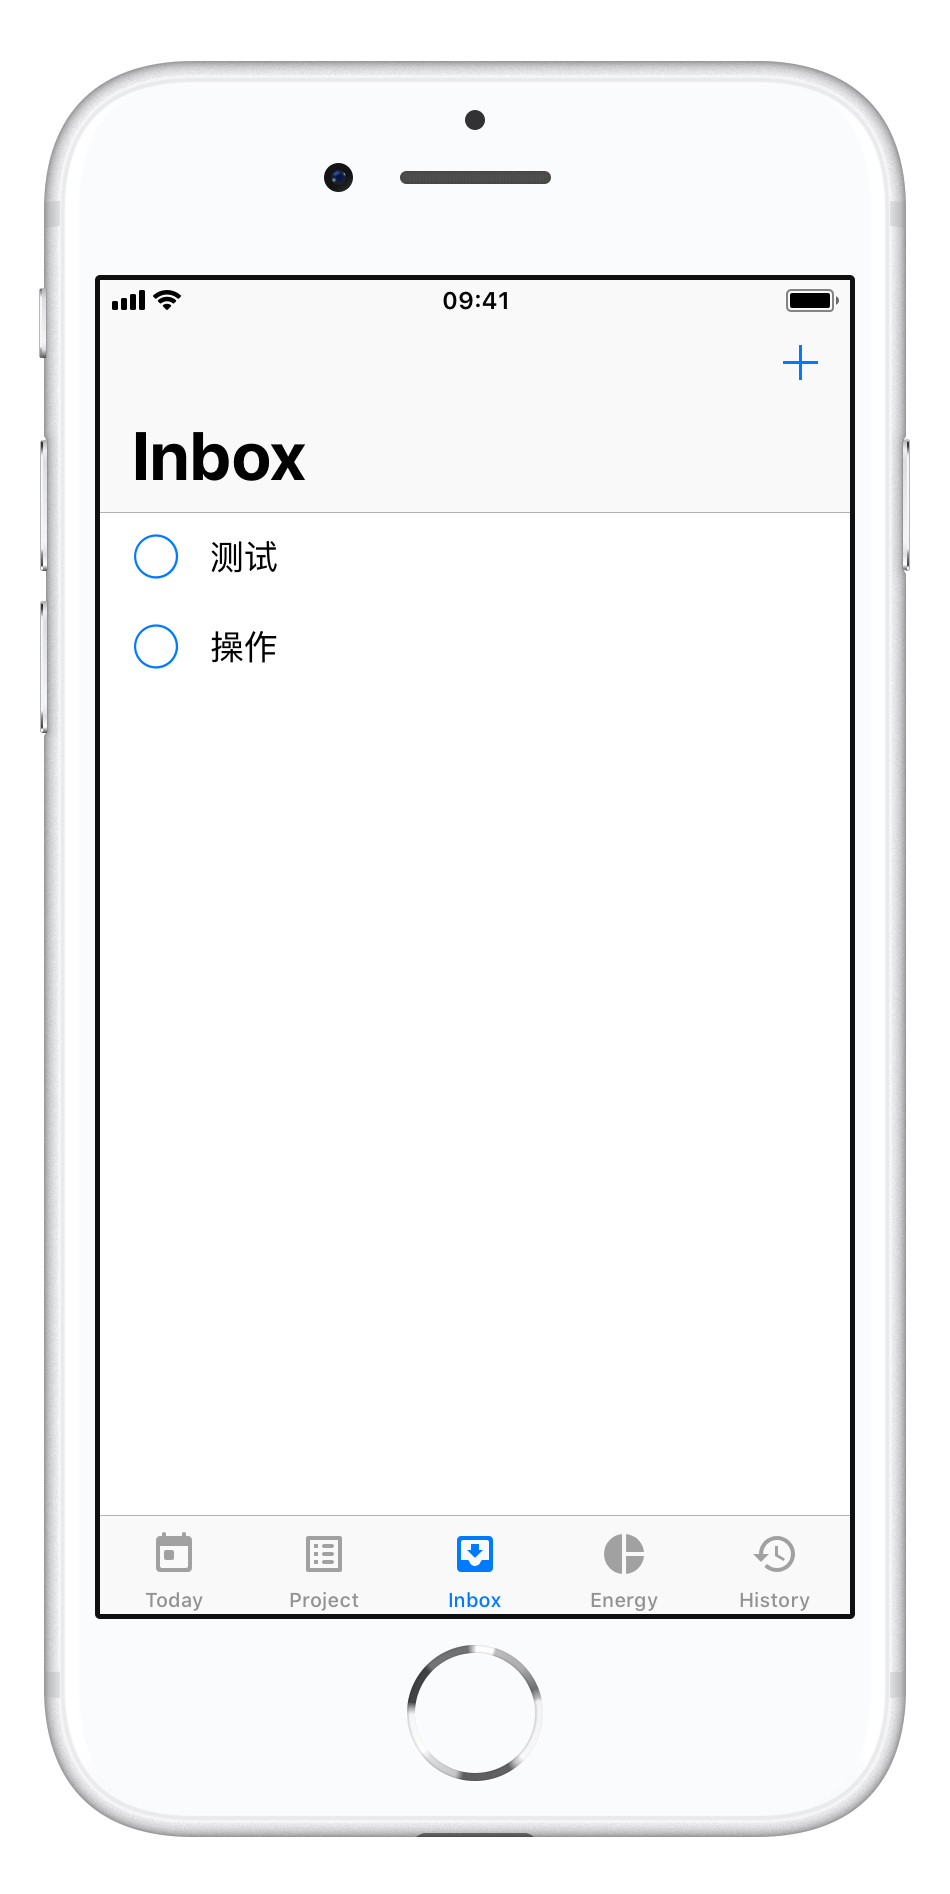
\includegraphics[height=10cm]{figure/system/inbox+no_split}}
	\caption{从系统提醒事项中拉取任务截图}
	\label{fig:inbox_no_split}
\end{figure}

对于任务是否完成,通过任务TableViewCell中左侧的图标来进行提示,并可以通过点击图标将任务标记为已完成,
根据MVC设计的原则由于TableViewCell本身并不了解任务的相关属性,自然也无从得知用户点击了哪一个任务的完成图标\parencite{ios2017program},
故需要通过代理告知TableViewController,由后者完成任务完成的相关操作。

\begin{lstlisting}[language={Swift}, caption={TaskTableViewCell}]
	@objc protocol TaskCellDelegate: class {
		func checkMarkTapped(sender: TaskTableViewCell)
	}

	class TaskTableViewCell: UITableViewCell {
		
		var delegate: TaskCellDelegate?
		
		@IBOutlet weak var doneProgressView: UIProgressView!
		
		@objc func imageViewTapped() {
			delegate?.checkMarkTapped(sender: self)
		}
		
		func update(with task: Task) {
			let color = task.project?.color as? UIColor
			textLabel?.text = task.title
			imageView?.image = task.isDone ? UIImage(named: "dot circle") : UIImage(named: "circle")
			imageView?.tintColor = color
			doneProgressView.isHidden = task.splitCount == 1
			doneProgressView.progressTintColor = color
			doneProgressView.trackTintColor = color?.withAlphaComponent(0.1)
		}
		
		override func awakeFromNib() {
			super.awakeFromNib()
			let leadingConstraint = NSLayoutConstraint.init(item: doneProgressView!, attribute: .leading, relatedBy: .equal, toItem: textLabel, attribute: .leading, multiplier: 1.0, constant: 0)
			self.addConstraints([leadingConstraint])
			imageView?.isUserInteractionEnabled = true
			let gesture = UITapGestureRecognizer(target: self, action: #selector(imageViewTapped))
			gesture.numberOfTapsRequired = 1
			imageView?.addGestureRecognizer(gesture)
		}
	}
\end{lstlisting}

~\\
~\\
\begin{lstlisting}[language={Swift}, caption={TaskListTableViewController实现代理的相关代码}]
	class TaskListTableViewController: UITableViewController, TaskCellDelegate {
		let context = AppDelegate.viewContext
		var store = EKEventStore()
		var tasks = [Task]()
		var sourceProject: Project? = nil
		...
		func checkMarkTapped(sender: TaskTableViewCell) {
        if let indexPath = tableView.indexPath(for: sender) {
            let task = tasks[indexPath.row]
            if task.splitCount == 1 {
                task.isDone = !task.isDone
                let action = Action(context: context)
                action.costMinutes = task.costMinutes
                action.doneTime = Date()
                action.doneUnitCount = 1
                action.energyLevel = task.energyLevel
                action.task = task
                try! context.save()
            }
            else {
                let sb = UIStoryboard(name: "Main", bundle: nil)
                let navViewController = sb.instantiateViewController(withIdentifier: "navAEAction") as! UINavigationController
                let vc = navViewController.topViewController as? AddEditActionTableViewController
                vc?.task = task
                present(navViewController, animated: true, completion: nil)
            }
            tasks[indexPath.row] = task
            tableView.reloadRows(at: [indexPath], with: .automatic)
		}
		...
    }
\end{lstlisting}

本系统的主要功能在于对任务进行详尽的设置,并通过相关的设置,对用户的任务完成情况,行为等进行跟踪和分析。
为了方便用户的设置,本系统尽可能的减少了用户的输入操作,改用DatePicker等便于输入的方式进行添加任务\parencite{app2019swift},
如图\ref{fig:add_task_duedate}所示。

\begin{figure}[H]
	\centering
	\makebox[\textwidth]{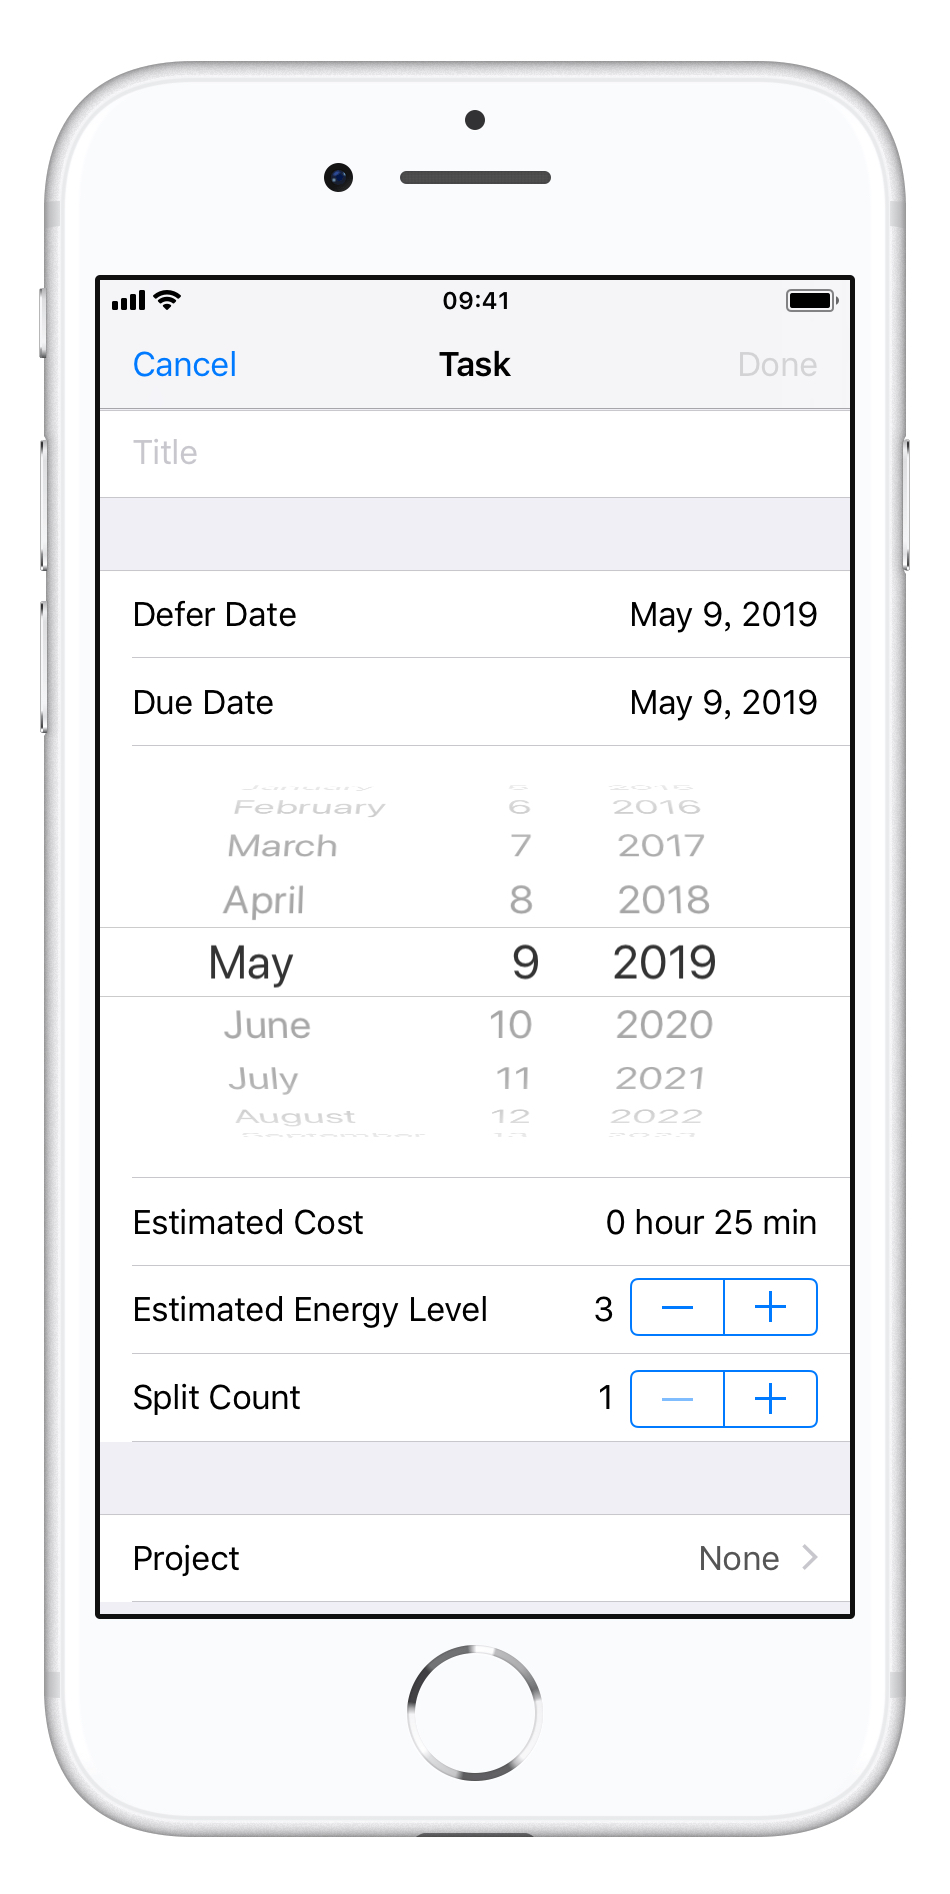
\includegraphics[height=10cm]{figure/system/add_task+duedate}}
	\caption{使用DatePicker添加到期日期}
	\label{fig:add_task_duedate}
\end{figure}

对于多个日期和表单的情况,通过代码动态控制TableView的行高来实现不同DatePicker的切换,代码如下。

\begin{lstlisting}[language={Swift}, caption={动态调整行高以便输入}]
	...
	let deferDatePickerCellIndexPath = IndexPath(row: 1, section: 1)
    let dueDatePickerCellIndexPath = IndexPath(row: 3, section: 1)
    let costTimePickerCellIndexPath = IndexPath(row: 5, section: 1)
    let splitUnitCellIndexPath = IndexPath(row: 8, section: 1)
    let projectCellIndexPath = IndexPath(row: 0, section: 2)
    let notesTextViewIndexPath = IndexPath(row: 0, section: 3)
    var isDeferDatePickerShown: Bool = false {
        didSet {
            deferDatePicker.isHidden = !isDeferDatePickerShown
        }
    }
    var isDueDatePickerShown: Bool = false {
        didSet {
            dueDatePicker.isHidden = !isDueDatePickerShown
        }
    }
    var isDurationTimePickerShown: Bool = false {
        didSet {
            costTimePicker.isHidden = !isDurationTimePickerShown
        }
    }
	...
	override func tableView(_ tableView: UITableView, didSelectRowAt indexPath: IndexPath) {
        tableView.deselectRow(at: indexPath, animated: true)
        view.endEditing(true)   // Hide Keyboard
        // Toggle DatePicker
        switch (indexPath.section, indexPath.row) {
        case (deferDatePickerCellIndexPath.section, deferDatePickerCellIndexPath.row - 1):
            isDeferDatePickerShown = !isDeferDatePickerShown
            isDueDatePickerShown = false
            isDurationTimePickerShown = false
            updateTableView()
            
        case (dueDatePickerCellIndexPath.section, dueDatePickerCellIndexPath.row - 1):
            isDeferDatePickerShown = false
            isDueDatePickerShown = !isDueDatePickerShown
            isDurationTimePickerShown = false
            updateTableView()
            
        case (costTimePickerCellIndexPath.section, costTimePickerCellIndexPath.row - 1):
            isDeferDatePickerShown = false
            isDueDatePickerShown = false
            isDurationTimePickerShown = !isDurationTimePickerShown
            updateTableView()
        
        default:
            break
        }
	}
	
	override func tableView(_ tableView: UITableView, heightForRowAt indexPath: IndexPath) -> CGFloat {
        // Define Date Picker height
        switch (indexPath) {
        case deferDatePickerCellIndexPath:
            return isDeferDatePickerShown ? 216.0 : 0.0
        
        case dueDatePickerCellIndexPath:
            return isDueDatePickerShown ? 216.0 : 0.0
        
        case costTimePickerCellIndexPath:
            return isDurationTimePickerShown ? 216.0 : 0.0
        
        case splitUnitCellIndexPath:
            return isSplitEnable ? 44.0 : 0.0
            
        case [projectCellIndexPath.section, projectCellIndexPath.row + 1],
             [projectCellIndexPath.section, projectCellIndexPath.row + 2]:
            return isProjectSelected ? 44.0 : 0.0
            
        case (notesTextViewIndexPath):
            return 180.0
        
        default:
            return 44.0
        }
    }
\end{lstlisting}

\subsection{项目管理模块}
项目管理的一个重要功能是能够选择项目中任务之间的依赖,
实现这一需求的解决方案是通过建立数据库中任务表到自身的关系。
并通过算法计算任务的所有依赖和所有后续,从而避免用户在选择依赖任务或后续任务时形成依赖环路\parencite{cormen2009introduction}。 

\begin{lstlisting}[language={Swift}, caption={计算任务依赖关系的代码}]
	extension Task {
		func getAllPrerequisites() -> Set<Task> {
			let selfPrerequisites = self.prerequisites as! Set<Task>
			if selfPrerequisites.isEmpty {
				return []
			} else {
				var childPrerequisites = Set<Task>()
				for prerequisite in selfPrerequisites {
					for task in prerequisite.getAllPrerequisites() {
						childPrerequisites.insert(task) }
				}
				return childPrerequisites.union(selfPrerequisites)
			}
		}
		func getAllDependents() -> Set<Task> {
			let selfDependents = self.dependents as! Set<Task>
			if selfDependents.isEmpty {
				return []
			} else {
				var childDependents = Set<Task>()
				for dependent in selfDependents {
					for task in dependent.getAllPrerequisites() {
						childDependents.insert(task) }
				}
				return childDependents.union(selfDependents)
			}
		}
	}
\end{lstlisting}

extension 是Swift中的一个语言特性,可以在不接触类源代码的情况下为类添加方法和计算属性。
由于本系统直接使用Core Data根据数据库的属性和表以及实体间的关系自动生成相关的类,且在Xcode中
默认并不可见,故使用extension 是比较方便和合适的做法。

为了实现代码和视图的重用,采用标示信息区别用户选择的任务性质,如图\ref{fig:select_prerequisites_tasks}。

\begin{figure}[!hbp]
	\centering
	\makebox[\textwidth]{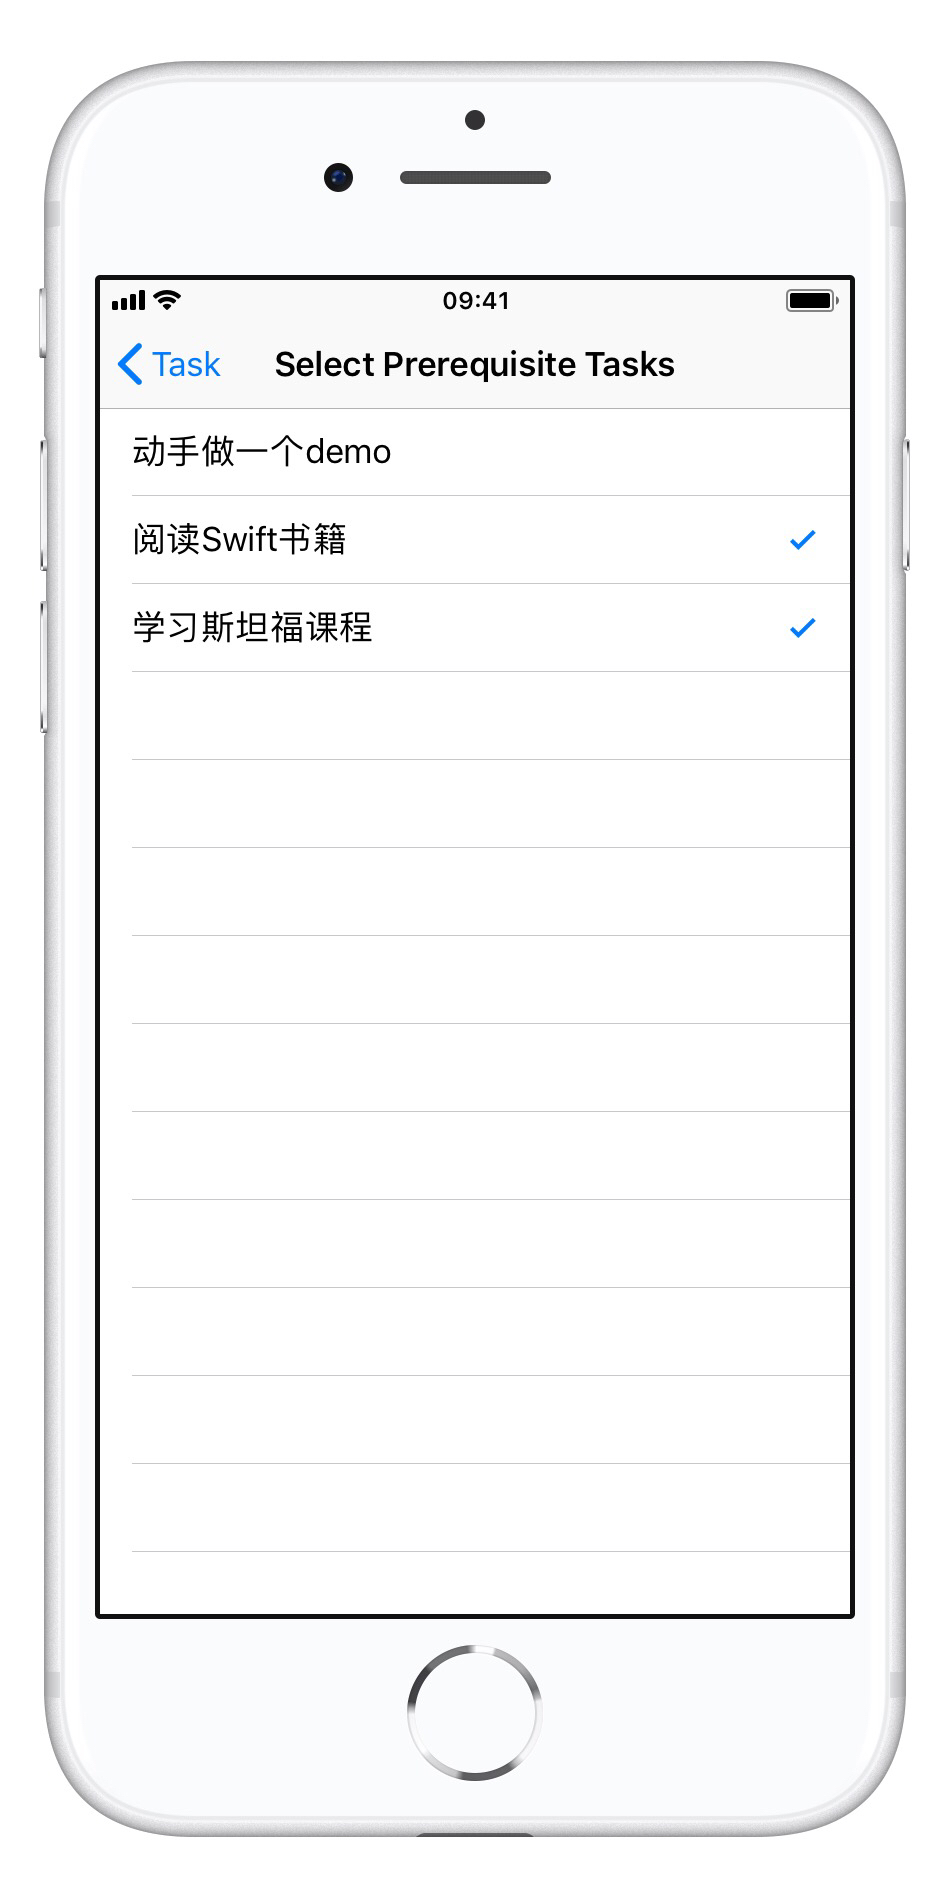
\includegraphics[height=10cm]{figure/system/select_prerequisites_tasks}}
	\caption{选择依赖任务}
	\label{fig:select_prerequisites_tasks}
\end{figure}

\begin{lstlisting}[language={Swift}, caption={选择任务界面的代码}]
class SelectTaskTableViewController: UITableViewController {

    let context = AppDelegate.viewContext
    var tasks = [Task]()
    var selectedTasks = [Task]()
    var identifier = ""
    
    override func viewWillDisappear(_ animated: Bool) {
        if isMovingFromParent {
            let navController = parent as! UINavigationController
            let addEditTaskTableViewController = navController.topViewController as! AddEditTaskTableViewController
            selectedTasks = []
            for i in 0..<tasks.count {
                let cell = tableView.cellForRow(at: [0,i])
                if cell?.accessoryType == .checkmark {
                    selectedTasks.append(tasks[i])
                }
            }
            switch identifier {
            case "SelectDependentTasks":
                addEditTaskTableViewController.dependentsTasks = selectedTasks
            case "SelectPrerequisiteTasks":
                addEditTaskTableViewController.prerequisiteTasks = selectedTasks
            default:
                break
            }
        }
    }
}
\end{lstlisting}

\subsection{精力管理模块}
本模块采用第三方库 AAChartView 效果如图\ref{fig:energy}所示。

\begin{figure}[!htbp]
	\centering
	\makebox[\textwidth]{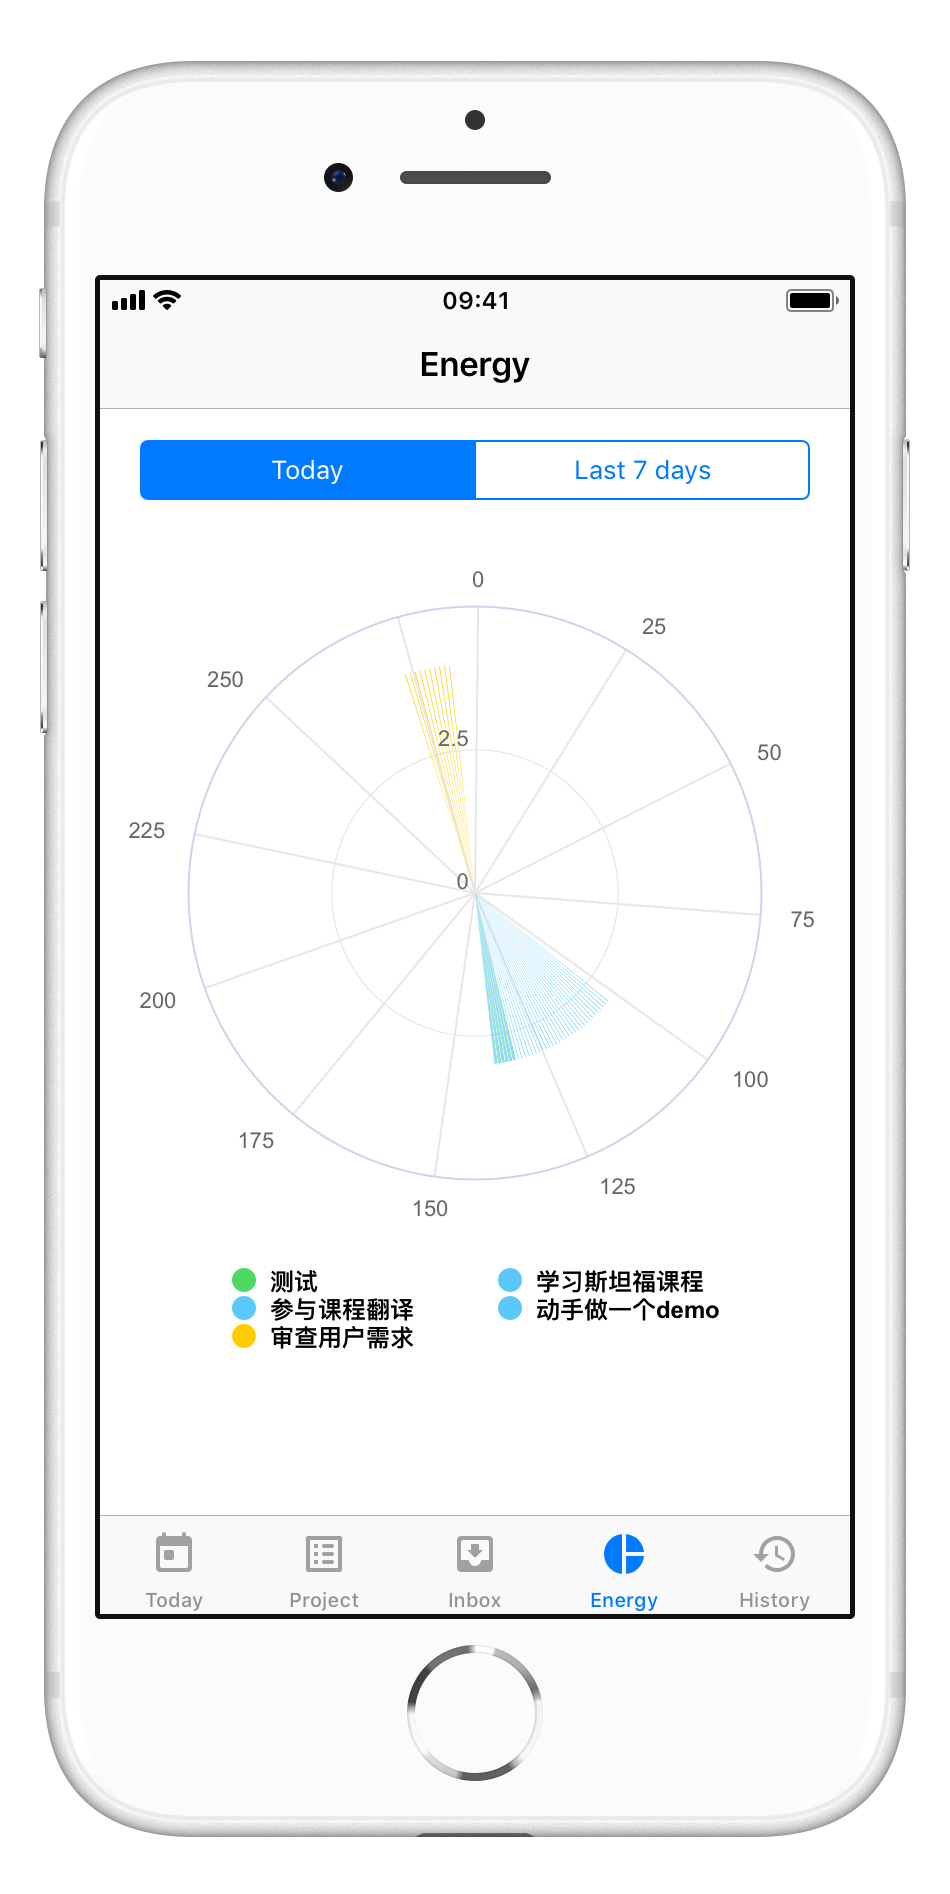
\includegraphics[height=10cm]{figure/system/energy}}
	\caption{查看精力极地图}
	\label{fig:energy}
\end{figure}

% \begin{lstlisting}[language={Swift}, caption={绘制极地图的代码}]
% var aaChartModel = AAChartModel()
% 	.chartType(chartType!)//图形类型
% 	.polar(true)
% 	.title("")
% 	.dataLabelEnabled(false)//是否显示数字
% 	.animationType(.bounce)//图形渲染动画类型为"bounce"

% var chartModelData = [[String : Any]]()

% var taskSet = Set<Task>()
% for action in actions {
% 	taskSet.insert(action.task!)
% }

% for task in taskSet {
% 	var data = Array(repeating: 0, count: 24*60/5)
% 	let actions = task.actions as? Set<Action>
% 	let calendar = Calendar.current
% 	for action in actions! {
% 		let dateComponents = calendar.dateComponents(in: calendar.timeZone, from: action.doneTime!)
% 		let end = (dateComponents.hour! * 60 + dateComponents.minute!) / 5
% 		let begin = end - Int(action.costMinutes/5)
% 		for i in begin...end {
% 			data[i] = Int(action.energyLevel)
% 		}
% 	}
% 	let color = task.project?.color as? UIColor
% 	let element = AASeriesElement()
% 	element.name(task.title!)
% 	element.color(color!.hexString!)
% 	element.data(data)
% 	chartModelData.append(element.toDic()!)
% }

% aaChartModel = aaChartModel.series(chartModelData)

% aaChartView?.aa_drawChartWithChartModel(aaChartModel)
% \end{lstlisting}

通过对行为完成时间的计算,以5分钟为间隔绘制相应时间段的用户精力情况。

\subsection{行为管理模块}

用户在完成任务时会自动添加相应的行为,对于被分割的任务,由于系统无法获知
用户具体完成情况,故弹出添加行为的窗口供用户选择完成的行为的相关信息,如图\ref{fig:add_action}。

\begin{figure}[!hbp]
	\centering
	\makebox[\textwidth]{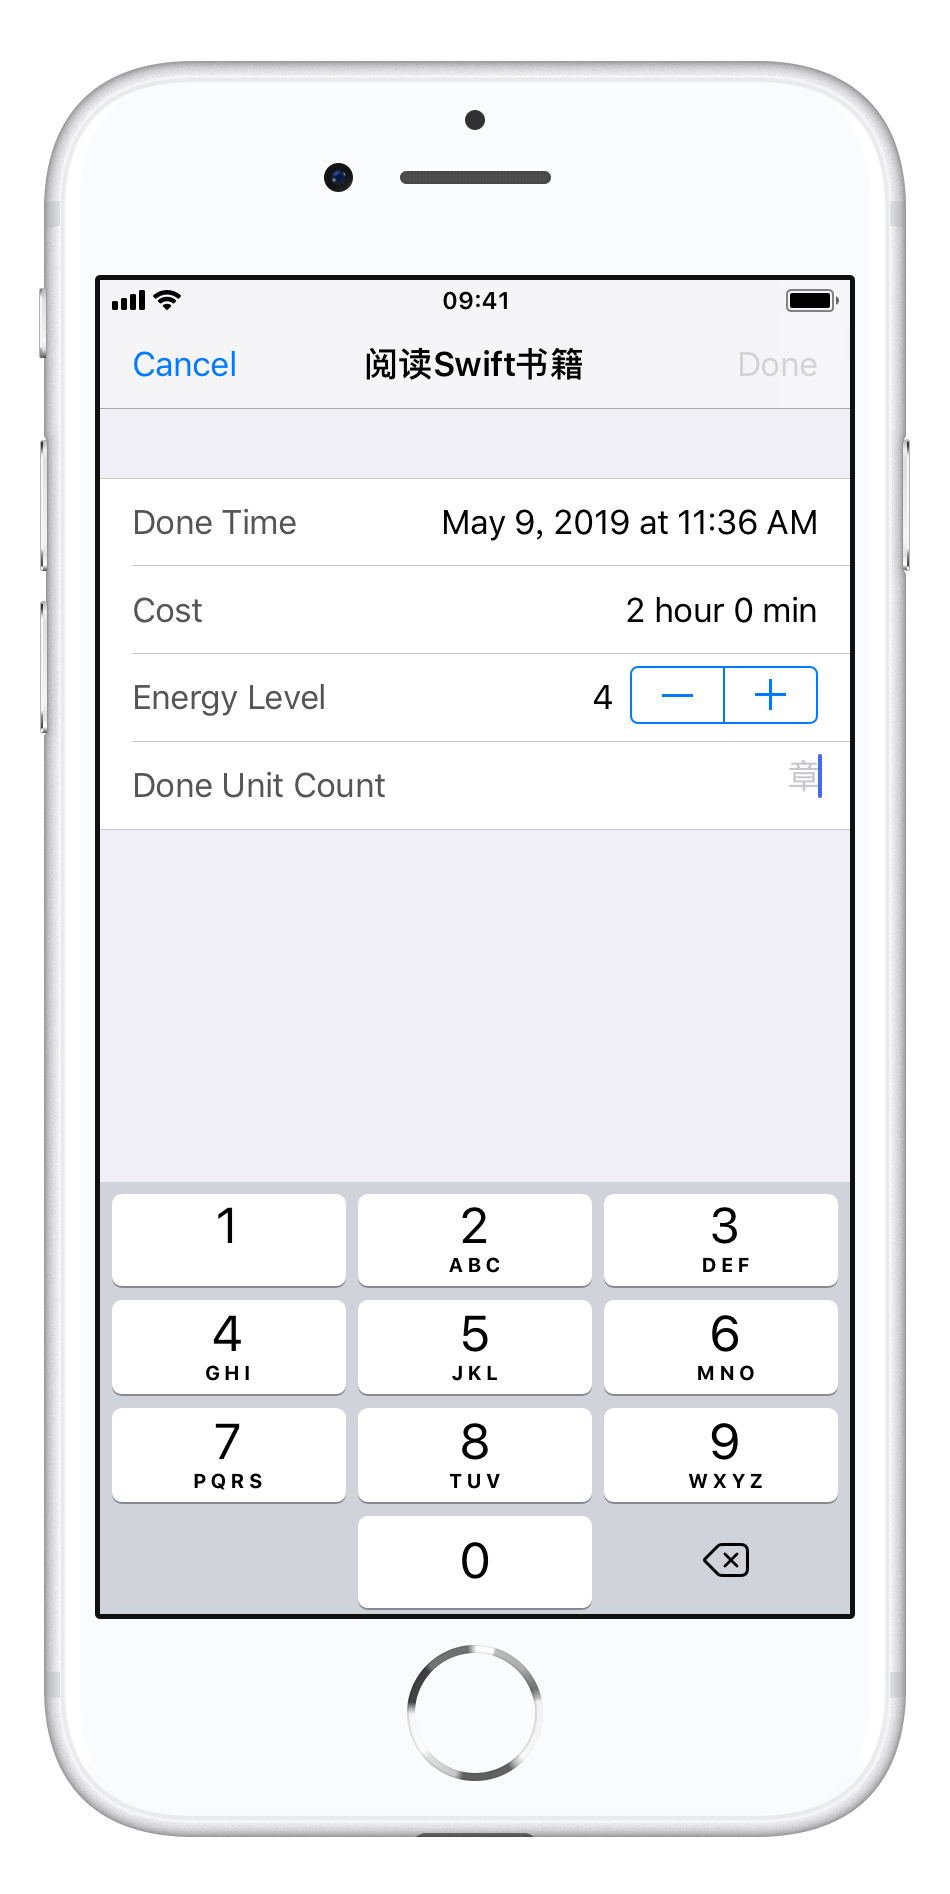
\includegraphics[height=10cm]{figure/system/add_action}}
	\caption{添加行为}
	\label{fig:add_action}
\end{figure}

\begin{lstlisting}[language={Swift}, caption={添加行为的代码}]
	override func tableView(_ tableView: UITableView, didSelectRowAt indexPath: IndexPath) {
        tableView.deselectRow(at: indexPath, animated: true)
        switch indexPath.row {
        case 0:
            let datePicker = doneTimeLabel.inputView as? UIDatePicker
            datePicker?.datePickerMode = .dateAndTime
            datePicker?.addTarget(self, action: #selector(doneDateTimePickerValueChanged(sender:)), for: .valueChanged)
            doneTimeLabel.becomeFirstResponder()
            datePicker?.setDate(doneTime, animated: true)
        case 1:
            let datePicker = costLabel.inputView as? UIDatePicker
            datePicker?.datePickerMode = .countDownTimer
            datePicker?.minuteInterval = 5
            datePicker?.addTarget(self, action: #selector(costTimePickerValueChanged(sender:)), for: .valueChanged)
            costLabel.becomeFirstResponder()
            datePicker?.countDownDuration = TimeInterval(costMinutes*60)
        case 3:
            doneUnitCountTextField.becomeFirstResponder()
        default:
            break
        }
    }
\end{lstlisting}

这一界面与iOS 的健康添加行为的界面保持一致,将键盘作为DatePicker等输入的入口,
更符合用户的操作习惯。

为了更方便的管理行为,还提供了历史记录的查看,如图\ref{fig:history}。

\begin{figure}[!htbp]
	\centering
	\makebox[\textwidth]{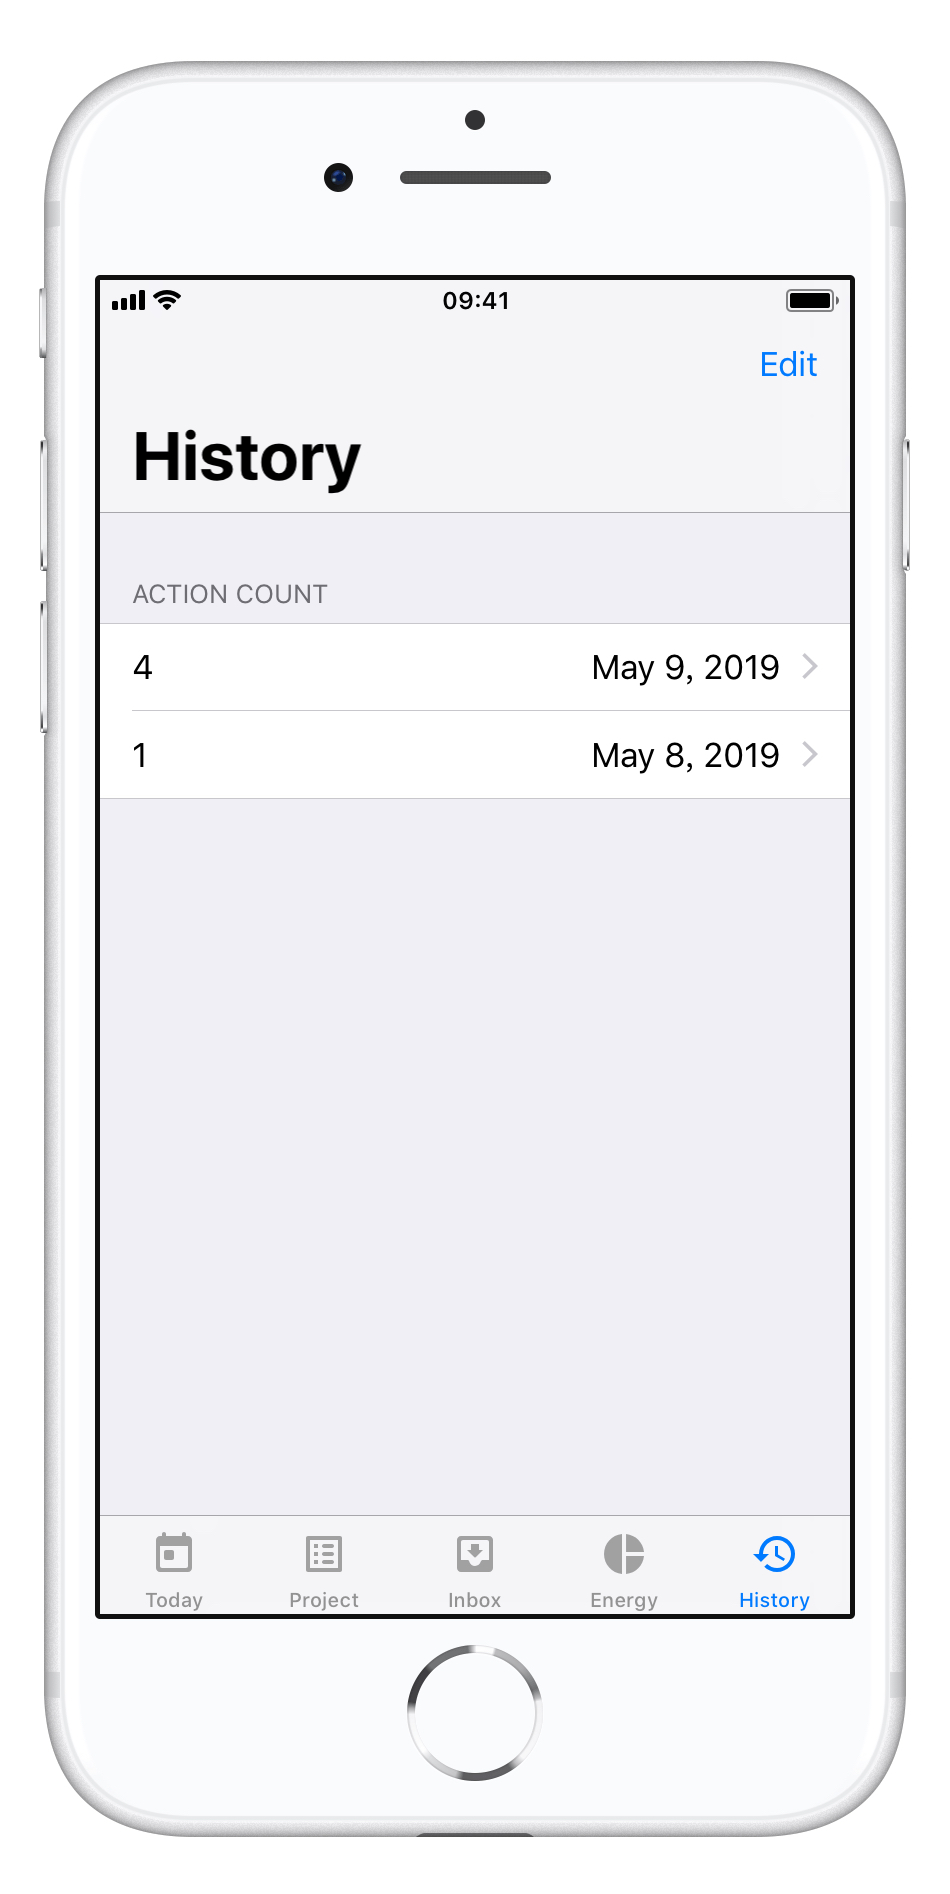
\includegraphics[height=10cm]{figure/system/history}}
	\caption{查看历史行为记录}
	\label{fig:history}
\end{figure}